%
% exemplo genérico de uso da classe iiufrgs.cls
% $Id: iiufrgs.tex,v 1.1.1.1 2005/01/18 23:54:42 avila Exp $
%
% This is an example file and is hereby explicitly put in the
% public domain.
%
\documentclass[ecp,tc]{iiufrgs}
% Para usar o modelo, deve-se informar o programa e o tipo de documento.
% Programas :
%   * cic       -- Graduação em Ciência da Computação
%   * ecp       -- Graduação em Ciência da Computação
%   * ppgc      -- Programa de Pós Graduação em Computação
%   * pgmigro   -- Programa de Pós Graduação em Microeletrônica
%   
% Tipos de Documento:
%   * tc                -- Trabalhos de Conclusão (apenas cic e ecp)
%   * diss ou mestrado  -- Dissertações de Mestrado (ppgc e pgmicro)
%   * tese ou doutorado -- Teses de Doutorado (ppgc e pgmicro)
%   * ti                -- Trabalho Individual (ppgc e pgmicro)
% 
% Outras Opções:
%   * english    -- para textos em inglês
%   * openright  -- Força início de capítulos em páginas ímpares (padrão da
%                   biblioteca)
%   * oneside    -- Desliga frente-e-verso
%   * nominatalocal -- Lê os dados da nominata do arquivo nominatalocal.def

\newcommand*{\captionsource}[2]{%
  \caption[{#1}]{#1}\par
  \textbf{Fonte:} #2\par
}


% Use unicode
\usepackage[utf8]{inputenc}   % pacote para acentuação

% Necessário para incluir figuras
\usepackage{graphicx}           % pacote para importar figuras


\usepackage{times}              % pacote para usar fonte Adobe Times
% \usepackage{palatino}
% \usepackage{mathptmx}          % p/ usar fonte Adobe Times nas fórmulas

\usepackage[alf,abnt-emphasize=bf]{abntex2cite}	% pacote para usar citações abnt

%
% Informações gerais
%
\title{Um Exemplo de Monografia do Instituto de Informática da UFRGS}

\author{Flaumann}{Fritz Gutenberg}
% alguns documentos podem ter varios autores:
%\author{Flaumann}{Frida Gutenberg}
%\author{Flaumann}{Klaus Gutenberg}

% orientador e co-orientador são opcionais (não diga isso pra eles :))
\advisor[Prof.~Dr.]{Lamport}{Leslie}
%\coadvisor[Prof.~Dr.]{Knuth}{Donald Ervin}

% a data deve ser a da defesa; se nao especificada, são gerados
% mes e ano correntes
%\date{maio}{2001}

% o local de realização do trabalho pode ser especificado (ex. para TCs)
% com o comando \location:
%\location{Itaquaquecetuba}{SP}

% itens individuais da nominata podem ser redefinidos com os comandos
% abaixo:
% \renewcommand{\nominataReit}{Prof\textsuperscript{a}.~Wrana Maria Panizzi}
% \renewcommand{\nominataReitname}{Reitora}
% \renewcommand{\nominataPRE}{Prof.~Jos{\'e} Carlos Ferraz Hennemann}
% \renewcommand{\nominataPREname}{Pr{\'o}-Reitor de Ensino}
% \renewcommand{\nominataPRAPG}{Prof\textsuperscript{a}.~Joc{\'e}lia Grazia}
% \renewcommand{\nominataPRAPGname}{Pr{\'o}-Reitora Adjunta de P{\'o}s-Gradua{\c{c}}{\~a}o}
% \renewcommand{\nominataDir}{Prof.~Philippe Olivier Alexandre Navaux}
% \renewcommand{\nominataDirname}{Diretor do Instituto de Inform{\'a}tica}
% \renewcommand{\nominataCoord}{Prof.~Carlos Alberto Heuser}
% \renewcommand{\nominataCoordname}{Coordenador do PPGC}
% \renewcommand{\nominataBibchefe}{Beatriz Regina Bastos Haro}
% \renewcommand{\nominataBibchefename}{Bibliotec{\'a}ria-chefe do Instituto de Inform{\'a}tica}
% \renewcommand{\nominataChefeINA}{Prof.~Jos{\'e} Valdeni de Lima}
% \renewcommand{\nominataChefeINAname}{Chefe do \deptINA}
% \renewcommand{\nominataChefeINT}{Prof.~Leila Ribeiro}
% \renewcommand{\nominataChefeINTname}{Chefe do \deptINT}

% A seguir são apresentados comandos específicos para alguns
% tipos de documentos.

% Relatório de Pesquisa [rp]:
% \rp{123}             % numero do rp
% \financ{CNPq, CAPES} % orgaos financiadores

% Trabalho Individual [ti]:
% \ti{123}     % numero do TI
% \ti[II]{456} % no caso de ser o segundo TI

% Monografias de Especialização [espec]:
% \espec{Redes e Sistemas Distribuídos}      % nome do curso
% \coord[Profa.~Dra.]{Weber}{Taisy da Silva} % coordenador do curso
% \dept{INA}                                 % departamento relacionado

%
% palavras-chave
% iniciar todas com letras minúsculas, exceto no caso de abreviaturas
%
\keyword{formatação eletrônica de documentos}
\keyword{\LaTeX}
\keyword{ABNT}
\keyword{UFRGS}

%
% inicio do documento
%
\begin{document}

% folha de rosto
% às vezes é necessário redefinir algum comando logo antes de produzir
% a folha de rosto:
% \renewcommand{\coordname}{Coordenadora do Curso}
\maketitle

% dedicatoria
\clearpage
\begin{flushright}
\mbox{}\vfill
{\sffamily\itshape
``If I have seen farther than others,\\
it is because I stood on the shoulders of giants.''\\}
--- \textsc{Sir~Isaac Newton}
\end{flushright}

% agradecimentos
\chapter*{Agradecimentos}
Aos meus pais, Ernesto Antônio Lando e Izidora Justina Bizotto Lando, e à minha irmã, Anelise Lando, que me apoiaram, acreditaram em mim e me deram suporte desde que saí de casa para vir morar sozinho em outro Estado para cursar Engenharia de Computação em uma das melhores universidades do país. Muito obrigado.

À Isadora, minha parceira de vida, que esteve ao meu lado nesses últimos anos, me apoiando, incentivando e ouvindo eu reclamar de tudo.
Muito obrigado, Isa, por toda essa parceria, conselhos e ajuda que você me deu. Eu evoluí muito como pessoa ao seu lado.

Ao Felipe Lando, meu irmão, que me acolhe desde as tentativas falhas do vestibular da UFRGS até hoje, juntamente com a minha cunhada, Amália Machado.
Muito obrigado por todos esses anos de parceria, muitos almoços, jantas e projetos que fizemos juntos desde que eu vim morar na Capital.
À Amália, um agradecimento especial por toda a ajuda que você me deu durante o desenvolvimento deste trabalho.
Se eu estou aqui hoje é principalmente graças a vocês dois e a Acadêmica Pesquisa.

Ao Urso, meu cachorro, que esteve ao meu lado durante todo o desenvolvimento deste trabalho, seja me mordendo, latindo, pulando por cima de mim querendo brincar ou só deitado em silêncio me fazendo companhia.
Eu sei que você não entende a importância do que eu estava fazendo, mas muito obrigado pelo carinho.

Aos meus colegas de trabalho da HP, que compreenderam as diversas vezes que precisei me ausentar para poder realizar atividades referentes a este trabalho.
Aqui vai um agradecimento especial à Thayná Minuzzo, que além de colega de trabalho, também foi minha colega durante a graduação, me ajudando em diversas disciplinas, incluindo dicas durante a realização do presente trabalho.
Vocês também tem uma parte desta minha conquista. Muito obrigado.

Aos meus colegas e amigos que estão comigo desde a primeira semana de aula, como a Ana e a Narumi, o Fischer, o Probst e o Rodrigo, além de outras amizades que eu fiz durante todos esses anos de graduação.
Vocês me confortaram, muitas vezes indiretamente, só de saber que todos nós estávamos passando pelas mesmas dificuldades durante toda a graduação, incluindo nesse trabalho.

Aos meus padrinhos e primos, Tia Enedina, Tio Ronei, Leonardo, Ramon, Lucas e Marina, que sempre me incentivaram e me acolheram nos feriados e finais de semana.
Muito obrigado por esse tempo juntos, me ajudaram a esfriar a cabeça nos momentos mais difíceis da graduação.

Ao meu orientador, Prof. Dr. Juliano Wickboldt, que me ofereceu a primeira oportunidade de bolsa de pesquisa, lá em 2017, no meu segundo semestre de graduação, com o Projeto FUTEBOL e, em 2021, aceitou ser meu orientador para o desenvolvimento desta pesquisa.
Aqui também vão meus agradecimentos aos bolsistas de iniciação científica do projeto PORVIR-5G, Lucas Schierholt e Mateus Milesi, que me ajudaram no desenvolvimento deste trabalho.
Sem vocês, eu não teria chegado até aqui.

Por fim, agradeço a todos aqueles que, de alguma forma, contribuíram para que este trabalho fosse concluído.
Espero que os resultados obtidos ajudem a desenvolver essa área da computação.



% resumo na língua do documento
\begin{abstract}
O presente trabalho desenvolve uma prova de conceito de um módulo para execução de testes de desempenho em implementações de núcleos de redes 5G.
O objetivo deste trabalho é analisar como se comportam as diferentes implementações de código aberto dos núcleos de rede 5G, \textit{free5GC}, \textit{Open5GS} e \textit{OpenAirInterface}, para a execução de procedimentos em escala.
Para responder a esse problema, primeiramente foi feito um um breve resumo sobre a evolução das redes móveis, com foco em implementações em software de núcleos de redes 5G.
A seguir, são apresentados os trabalhos relacionados, assim como as diferenças entre eles e a presente pesquisa.
Após, uma arquitetura de software foi desenvolvida, criando um módulo de extensão para o testador \textit{my5G-RANTester} para realizar testes de desempenho nessas implementações de código aberto de núcleos de redes 5G.
Foram executados experimentos sobre essas implementações.
Na primeira fase dos experimentos, foi feito um teste para analisar o tempo médio de conexão de cada equipamento de usuário com cada núcleo testado. Na segunda etapa do experimento, foi medida a largura de banda do plano de dados entre o equipamento de usuário e o núcleo da rede.
Dentre os principais resultados obtidos, foi possível observar que o \textit{free5GC} apresenta melhor desempenho em relação à largura de banda disponível para os equipamentos de usuário, enquanto que o \textit{Open5GS} apresenta mais estabilidade durante o processo de registro de múltiplos equipamentos de usuário.
Este trabalho possui duas importantes contribuições teóricas para a literatura. A primeira contribuição é a agregação de conhecimento sobre testes de desempenho em redes móveis, enquanto a segunda é relacionada com a estabilidade e limitações das implementações de núcleos 5G em software.
A principal contribuição prática deste trabalho é o desenvolvimento de um módulo para realizar testes de desempenho em núcleos de rede 5G.
Como sugestões de futuras pesquisas, é possível avançar a investigação sobre experimentos em núcleos comerciais ou replicar os testes em ambientes de fácil escalabilidade.


\end{abstract}

% resumo na outra língua
% como parametros devem ser passados o titulo e as palavras-chave
% na outra língua, separadas por vírgulas
\begin{englishabstract}{Title in English}{Keywords}
The present work develops a proof of concept of a module to run performance tests on 5G network core implementations.
The main goal of this work is to analyze how the different open source implementations of the 5G network cores behave, such as free5GC, Open5GS and OpenAirInterface, for the execution of procedures at scale.
To answer this problem, a brief summary of the evolution of mobile networks was made, focusing on software implementations of 5G network cores.
Next, the related works are presented, as well as the differences between them and the present research.
Afterwards, a software architecture was developed, creating an extension module for the my5G-RANTester to run performance tests on these open source implementations of 5G network cores.
Experiments were performed on these implementations.
In the first phase of the experiments, a test was carried out to analyze the average connection time of each user equipment with each tested core. In the second stage of the experiment, the data plane throughput between the user equipment and the network core was measured.
Among the main results obtained, it was possible to observe that free5GC presents better performance in relation to the throughput available to user equipments, while Open5GS presents more stability during the registration process of multiple user equipments.
This work has two important theoretical contributions to the literature. The first contribution is the aggregation of knowledge about performance testing in mobile networks, while the second is related to the stability and limitations of 5G core implementations in software.
The main practical contribution of this work is the development of a module to run performance tests on 5G network cores.
As suggestions for future research, it is possible to advance the investigation on experiments in commercial cores or to replicate the tests in easily scalable environments.
\end{englishabstract}

% lista de abreviaturas e siglas
% o parametro deve ser a abreviatura mais longa
\begin{listofabbrv}{SPMD}
        \item[SMP] Symmetric Multi-Processor
        \item[NUMA] Non-Uniform Memory Access
        \item[SIMD] Single Instruction Multiple Data
        \item[SPMD] Single Program Multiple Data
        \item[ABNT] Associação Brasileira de Normas Técnicas
\end{listofabbrv}

% idem para a lista de símbolos
%\begin{listofsymbols}{$\alpha\beta\pi\omega$}
%       \item[$\sum{\frac{a}{b}}$] Somatório do produtório
%       \item[$\alpha\beta\pi\omega$] Fator de inconstância do resultado
%\end{listofsymbols}

% lista de figuras
\listoffigures

% lista de tabelas
\listoftables

% sumario
\tableofcontents

% aqui comeca o texto propriamente dito

% introducao
\chapter{Introdução}
\label{sec:intro}
\input{TG2/Chapters/1.Introduction}

\chapter{Fundamentação teórica}
\label{sec:background}
\section{Primeiras gerações de redes móveis}

Devido à complexidade das redes móveis modernas, conhecer a evolução dessas redes se torna necessário para facilitar o seu entendimento. Originalmente, as redes móveis tinham o foco em comunicações de voz analógica, sendo uma extensão da rede de telefonia pública \textit{(Public Switched Telephone Network - PSTN)}, que operava com rede de roteamento de circuitos \cite{Cardoso2020}.
Entretanto, essas redes móveis foram adaptadas para transporte de dados com taxas de transmissão muito baixas, atingindo velocidades de até 2.4 kbps. Essas redes ficaram conhecidas como rede móvel de primeira geração (1G) \cite{vora2015evolution}.

Com a necessidade de evoluir as redes 1G, surge a segunda geração (2G), que provia um sinal com melhor qualidade, maiores taxas de transferência de dados e maior aproveitamento do espectro das ondas de rádio.
Todavia, essa tecnologia ainda mantinha seu foco em roteamento de circuitos.
Nessa geração, também surge o serviço de troca de mensagens curtas, conhecido como \textit{Short Message Service} (SMS).
Foi no 2G que a tecnologia de transporte de dados \textit{Global System for Mobile Communications} (GSM) foi inserida \cite{bhalla2010generations}.

Em 1998, inicia-se a parceria entre diversas organizações responsáveis pela criação dos padrões de telecomunicação denominada 3GPP\footnote{\url{https://www.3gpp.org/about-3gpp}}, que publica a \textit{Release 1999} no início do ano 2000.
Em redes móveis, \textit{releases} são conjuntos de recursos e especificações disponibilizadas a cada período, definindo os padrões a serem seguidos para a implementação dessas redes.
A \textit{Release 1999} descreve uma nova tecnologia de redes móveis, com foco em roteamento de pacotes.
Porém, essa tecnologia mantinha a compatibilidade com as tecnologias antigas, sendo denominada redes móveis de terceira geração (3G) \cite{3gpp.01.01}.

Inicialmente, o padrão definido para as redes 3G foi o \textit{Wide-Band Code-Divison Multiple Access} (WCDMA).
Entretanto, em 2002, o início do desenvolvimento do padrão \textit{High-Speed Downlink Packet Access} (HSDPA) é anunciado, suportando velocidades de transmissão teóricas de até 14 Mbps. Isso permitiria navegação na internet mais rápida, acesso a conteúdos de televisão diretamente no aparelho celular e chamadas de vídeo. O padrão HSDPA foi chamado de 3.5G e teve a sua especificação finalizada em 2004 \cite{Lamba2012}.

No final de 2008, a \textit{Release 8} é publicada pela 3GPP, especificando os requisitos para a tecnologia \textit{Long Term Evolution} (LTE), que viria para substituir a terceira geração de redes móveis.
Entretanto, essa especificação não preenchia os requisitos mínimos para ser considerada uma quarta geração de redes móveis, sendo assim conhecida como 3.9G \cite{delperal2018}.
Dentre as mudanças provindas desta nova tecnologia, é importante mencionar a remoção do suporte à roteamento de circuitos, fazendo com que essa geração usasse apenas roteamento de pacotes sobre IP para todo o tráfego de informações na rede.

Toda a informação de áudio de ligações telefônicas era trafegada sobre a rede de roteamento de circuitos nas gerações anteriores ao LTE.
Com a remoção dessa tecnologia no LTE, foi necessário desenvolver um novo protocolo, surgindo assim o \textit{Voice over LTE} (VoLTE).
O VoLTE, assim como a tecnologia \textit{Voice over IP} (VoIP), trafega os dados de voz de ligações telefônicas sobre a rede de roteamento de pacotes, permitindo que as operadoras de redes móveis pudessem continuar oferecendo o serviço de ligações telefônicas para seus clientes. Nesta época, esse serviço era o mais rentável para as operadoras \cite{Yi2012}. 

Visando preencher os requisitos mínimos para a criação da quarta geração de redes móveis (4G), no início de 2011 é publicada a \textit{Release 10} pela 3GPP, criando assim a tecnologia \textit{LTE-Advanced} (LTE-A) \cite{3gpp.21.201}.
O 4G prometia velocidades de \textit{download} de pico de até 1Gbps e velocidades de \textit{upload} de pico de até 100Mbps.
Atingir tais velocidades só era possível graças à remoção do suporte ao roteamento de circuitos que ocorreu no 3.9G.

Antes do surgimento do LTE, existiam apenas 3 componentes na rede. Um era o equipamento de usuário, denominado \textit{User Equipment} (UE), sendo esse o dispositivo móvel. Outro componente era a rede de acesso via rádio, ou \textit{Radio Access Network} (RAN), denominada na tecnologia 3G de \textit{Universal Mobile Telecommunications System (UMTS) Terrestial Radio Network} (UTRAN), que englobava a estação de rádio base, chamada de \textit{Node B} (NB). Por fim, o terceiro componente era o núcleo da rede, ou \textit{Core Network} (CN), que no 3G era denominado \textit{UMTS Core Network} \cite{Miah2002}.
No entanto, a especificação da rede LTE trouxe uma melhor separação dos seus componentes do núcleo da rede, denominado \textit{Evolved Packet Core} (EPC) nessa geração, além de renomear a RAN para \textit{Evolved UTRAN} (E-UTRAN), chamando a estação base de \textit{Evolved Node B} (eNodeB).
O EPC foi separado em 4 elementos, sendo eles o \textit{Serving Gateway (Serving GW)}, o \textit{Packet Data Network Gateway (PDN GW)}, o \textit{Mobility Management Entity} (MME) e o \textit{Home Subscriber Server} (HSS) \cite{3gpp.23.214}.

\section{Redes 5G}

Em 2017, a 3GPP publica a versão inicial da \textit{Release 15}, com as definições da quinta geração de redes móveis, o 5G \cite{3gpp.21.205}.
Assim como nas gerações anteriores, o 5G visava introduzir melhorias na capacidade de transmissão de dados da RAN e redução da latência de comunicação entre o UE e a RAN.
Entretanto, essa geração teve como objetivo criar uma rede mais dinâmica e com maior flexibilidade em relação ao LTE.
Nessa geração também houve a integração com tecnologias de comunicação sem fios não-3GPP, que enquadram dispositivos denominados de \textit{Internet of Things} (IoT).

A \textit{Release 15} também introduziu as arquiteturas de rede 5G \textit{Non-Stand Alone} (NSA) e 5G \textit{Stand Alone} (SA).
Na arquitetura NSA, o núcleo da rede 4G é utilizado para a autenticação e comunicação dos dispositivos 5G, substituindo-se a E-UTRAN pela \textit{5G New Radio} (5GNR) e, consequentemente, a eNodeB pela gNodeB.
A rede NSA é considerada uma rede de transição entre o 4G e o 5G, pois o custo de implementação é baixo em ambientes onde já existe cobertura 4G das operadoras.

Por outro lado, a arquitetura SA introduziu um novo núcleo da rede, denominado de \textit{5G Core} (5GC).
De acordo com a especificação da 3GPP, o 5GC é um conjunto de componentes interconectados através de uma camada de serviços. Cada componente tem seu grupo específico de responsabilidades por consumir e prover serviços de e para outros elementos do sistema 5G, através de uma \textit{Application Programming Interface} (API).

A quinta geração de redes móveis também trouxe uma nova arquitetura do núcleo da rede, ilustrada em alto nível na Figura \ref{fig:5Gcore}. Os principais componentes dessa rede são o \textit{Access and Mobility Management Function} (AMF), o \textit{Session Management Function} (SMF) e o \textit{User Plane Function} (UPF).
O AMF é responsável por garantir que o processo de comunicação ocorra de maneira coesa e transparente, considerando a mobilidade do usuário como principal fator.
O SMF é responsável por estabelecer, modificar e liberar as sessões de cada equipamento de usuário, além de requisitar a alocação de um endereço de IP para esses UEs.
O UPF é o responsável pelo processamento e encaminhamento dos dados provindos dos UEs. Esses componentes serão discutidos com maior profundidade na subseção \ref{sub:components}.

\begin{figure}[!ht]
    \centering
    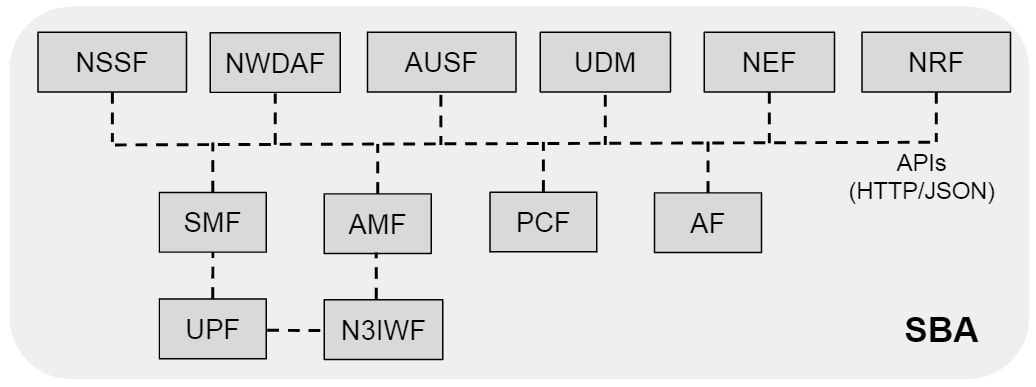
\includegraphics[width=1\textwidth]{TG2/Chapters/Background/Figures/Background-Core5G.png}
    \captionsource{Core 5G software components.}{\cite[p.~15]{Cardoso2020}}
    \label{fig:5Gcore}
\end{figure}

Os demais nove componentes do núcleo do 5G realizam uma variedade de funções.
O \textit{Authentication Server Function} (AUSF) é a função responsável por prover os serviços de autenticação dos UEs.
O \textit{Unified Data Management} (UDM) gerencia as informações dos usuários conectados na rede.
O \textit{Network Repository Function} (NRF) é um repositório que lista todas as funções de rede disponíveis em sua instância do núcleo do 5G.
O \textit{Policy Control Function} (PCF) é o responsável por controlar o comportamento da rede, aplicando políticas de segurança e controle.
O \textit{Network Slice Selection Function} (NSSF) é o componente responsável por controlar os \textit{slices} da rede para cada UE.
O \textit{Network Exposure Function} (NEF) é responsável por expor eventos internos relacionados aos UEs.
O \textit{Network Data Analytics Function} (NWDAF) é a função responsável por coletar e analisar dados provindos dos outros componentes da rede, incluindo informações dos usuários.
O \textit{Application Function} (AF) é um componente genérico que interage com os outros componentes no intuito de melhorar a qualidade do serviço para o usuário.
O \textit{Non-3GPP InterWorking Function} (N3IWF) é o responsável por integrar dispositivos não-3GPP com a rede 5G.

\subsection{Protocolos NAS e NGAP e Sessões de PDU}

Os protocolos \textit{Non-Access Stratum} (NAS) e \textit{NG Application Protocol} (NGAP) são essenciais para a comunicação entre o núcleo da rede, a RAN e o UE através do plano de controle.
As sessões de \textit{Packet Data Unit} (PDU) são importantes para garantir o funcionamento do plano de usuário da rede 5G.
A Figura \ref{fig:5Gprotocols} representa a arquitetura de uma rede 5G, exibindo os protocolos NAS e NGAP e as sessões de PDU entre o equipamento de usuário, a gNodeB e o núcleo da rede.

\begin{figure}[!ht]
    \centering
    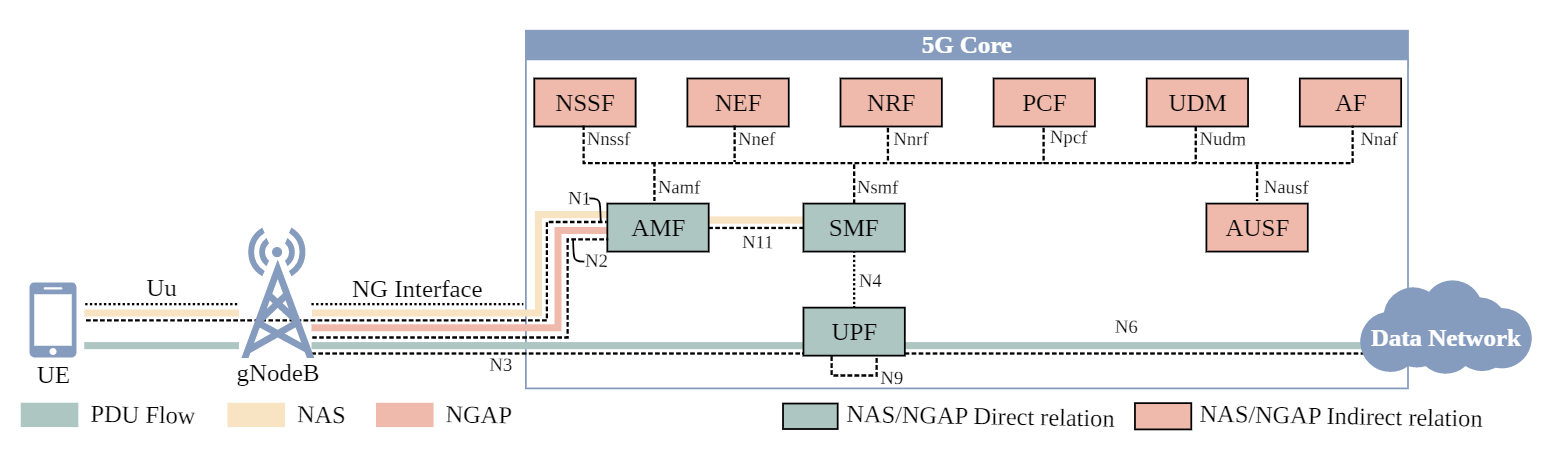
\includegraphics[width=1\textwidth]{TG2/Chapters/Background/Figures/Background-5GSystemProtocols.png}
    \captionsource{5G Core (5GC) Service-based Architecture (SBA).}{\cite[p.~3]{Dominato2021}}
    \label{fig:5Gprotocols}
\end{figure}

O protocolo NAS é usado para fazer a comunicação entre o UE e a função do núcleo AMF, tanto para dispositivos 3GPP quanto não-3GPP. A principal função do protocolo NAS é dar suporte à mobilidade do equipamento de usuário, incluindo procedimentos como autenticação, identificação e atualização das configurações genéricas do UE. O NAS também é responsável por suportar os procedimentos de gerenciamento de sessões, para estabelecer e manter a conexão de dados entre o UE e a rede de dados \cite{3gpp.24.501}. Esse protocolo também é o responsável por fazer a autenticação e gerenciar a conexão da gNodeB com o núcleo da rede.

O protocolo NGAP é o protocolo padrão para a comunicação do plano de controle entre a RAN e o núcleo da rede. O NGAP suporta os procedimentos de gerenciamento de interfaces, transporte das mensagens do protocolo NAS, gerenciamento de contexto do UE e das sessões de PDU. O gerenciamento de interfaces é o responsável por estabelecer e manter a conexão entre os componentes do núcleo da rede, onde as mensagens dos protocolos NAS e NGAP são transportados. O Protocolo NGAP é responsável por encapsular e transportar as mensagens NAS, provindas do UE, entre a RAN e o AMF. O gerenciamento de contexto do UE provê informações dos UEs para a RAN, como informações de segurança, lista de restrições de mobilidade e capacidade do rádio do UE. O gerenciamento das sessões de PDU é responsável por gerenciar os fluxos das unidades de pacotes de dados entre o núcleo da rede e a RAN, estabelecendo a interface de rádio utilizada para tráfego de controle e dados dos UEs \cite{3gpp.38.413}.

As sessões de PDU são responsáveis por prover a conexão fim-a-fim para o plano de usuário entre o UE e a rede de dados externa, através da função de rede UPF.
O fluxo de dados trafegado através das sessões de PDU é chamado de fluxo PDU e seus pacotes de dados são encapsulando sobre o protocolo de rede \textit{User Datagram Protocol} (UDP) \cite{3gpp.38.415}.

\subsection{Principais componentes da Rede 5G}
\label{sub:components}

Dentro do núcleo da rede, os componentes AMF, SMF e UPF são os responsáveis por gerenciar todo o tráfego de informações provindos da RAN.
O AMF é a porta de entrada do núcleo da rede em relação ao plano de controle.
Sendo assim, todo o tráfego dos protocolos NAS e NGAP provindos da RAN é direcionado para essa função do núcleo da rede.
Quando uma nova gNodeB inicia o processo de conexão com um núcleo existente, a autenticação e o estabelecimento da conexão é feito através de mensagens trocadas que utilizam o protocolo NAS entre a RAN e o AMF.
Após estabelecida a conexão, uma mensagem é enviada da RAN para o SMF, indiretamente através do AMF, utilizando o protocolo NAS, para que o SMF tenha conhecimento da gNodeB e possa gerenciar sua sessão.

Estando a RAN operacional, dispositivos 3GPP e não-3GPP dentro da área de cobertura da antena poderão iniciar sua conexão com essa rede 5G. Um dispositivo 3GPP, ao iniciar a conexão com essa rede 5G, troca mensagens com a RAN através do protocolo NAS. A RAN encapsula essas mensagens para o protocolo NGAP e encaminha para o núcleo da rede. O AMF, comunicando-se com os demais componentes da rede, autentica o UE através de um fluxo de informações definido na \textit{Release 15} do 3GPP \cite{3gpp.29.509}. Após concluir a autenticação do UE, o SMF se torna o responsável por gerenciar a sessão do equipamento de usuário. Um fluxo de dados PDU é estabelecido entre o UE e a função do núcleo UPF, que é responsável por gerenciar e encaminhar os pacotes de dados provindos dos UEs.

O UPF é a função do núcleo da rede 5G responsável por ser o ponto de conexão do núcleo da rede com qualquer rede externa.
É o UPF que encaminha os pacotes de dados provindos do UE através das sessões de PDU para a rede externa, sendo o responsável pelo roteamento de pacotes entre a rede externa e os diversos UEs conectados nessa rede 5G.
Essa função do núcleo da rede 5G aloca os endereços de IP para os UEs quando requisitado pelo SMF \cite{3gpp.23.501}.
O UPF também é responsável por coletar métricas de qualidade de serviço (QoS) do plano de usuário que serão usadas na função NWDAF \cite{3gpp.23.548}.

\section{Testes em rede móveis definidas por software}

Segundo \cite[p.~2, tradução nossa]{Bertolino2003}, ``teste de software consiste na verificação dinâmica do comportamento de um programa em um conjunto finito de casos de teste, adequadamente selecionados do domínio de execuções geralmente infinitas, em relação ao comportamento esperado especificado".
Com relação ao comportamento das redes sem fios implementadas em software, é importante executar testes para garantir que o funcionamento da rede esteja dentro do esperado.
Dentre os tipos de testes que podem ser executados em cima de implementações de redes 5G \textit{open source}, os que se destacam são os testes de conformidade, robustez e desempenho, como descrito em \cite{Dominato2021} e \cite{Zhang2019ASO}.

\subsection{Testes de Conformidade}

De acordo com \cite{Sarikaya1989}, teste de conformidade é definido como a atividade de teste realizada com o objetivo de verificar as capacidades e o comportamento de uma implementação em teste em relação aos requisitos de conformidade fornecidos no padrão de protocolo.
Os resultados dos testes de conformidade são do tipo lógico, sendo verdadeiro no caso onde a implementação em teste seja aprovada e falso no caso contrário.
Dessa forma, o uso de testes de conformidade em redes 5G é importante para verificar se a implementação da rede móvel se comporta de acordo com a especificação da 3GPP em casos onde o equipamento de usuário execute corretamente as operações descritas.

\cite{Rayner1987} divide o grupo de testes de conformidade em quatro categorias: testes básicos de interconexão, testes de capacidade, testes de comportamento e testes de resolução de conformidade.
Os testes básicos de interconexão são feitos para detectar quaisquer casos graves de não conformidade com a especificação do sistema.
Os testes de capacidade verificam se as capacidades observáveis da implementação em teste estão de acordo com os requisitos de conformidade estática da especificação. Os testes de conformidade estática são executados sobre o código fonte da aplicação.
Os testes de comportamento verificam a implementação da forma mais abrangente possível para ver se a implementação está de acordo com os requisitos de conformidade dinâmica da especificação. Os testes de conformidade dinâmica são realizados durante ou após a execução da implementação.
Os testes de resolução de conformidade examinam em profundidade requisitos específicos na implementação, verificando se a implementação se comporta exatamente como a especificação destes requisitos.

\subsection{Testes de Robustez}

Segundo \cite[p.~64, tradução nossa]{IEEE.Standard.Glossary}, robustez é definida como ``o grau em que um sistema ou componente pode funcionar corretamente na presença de entradas inválidas ou condições ambientais estressantes".
Os resultados dos testes de robustez também são do tipo lógico, sendo verdadeiro no caso onde a implementação em teste seja aprovada e falso no caso contrário.
Sendo assim, o teste de robustez no núcleo de redes móveis verifica o comportamento da rede em situações atípicas. \cite{Dominato2021} dividem o grupo de testes de robustez em um subgrupo de testes, que envolve testes de registro, de autenticação e de segurança, além de testes específicos para cada protocolo e função de rede do núcleo que serão detalhados na Subseção \ref{subsec:Dominato}.

\subsection{Testes de Desempenho}

Os testes de desempenho são importantes para validar o funcionamento da rede em uma carga alta de trabalho, o que representa uma situação de sobrecarga de uso da rede, o que pode causar mal funcionamento da rede e, em situações mais críticas, uma interrupção total do serviço.
Para a execução de testes de desempenho, costuma-se usar aplicações de referência, chamados de \textit{benchmarks}.
Os \textit{softwares} de \textit{benchmark} são aqueles que utilizam os mesmos parâmetros de entrada para avaliar o desempenho de diferentes sistemas ou serviços \cite{Boano2018}.
Sendo assim, o usuário pode comparar as métricas obtidas na execução com métricas coletadas de outras execuções em diferentes sistemas ou serviços e avaliar o desempenho do teste.

Para a avaliação dos testes de desempenho em redes móveis em software, \cite{Lee2021} utilizam dois grupos de métricas.
O primeiro grupo engloba métricas de desempenho de rede: taxa de transferência de dados, latência e perda de pacotes.
O segundo grupo é composto por métricas de desempenho de \textit{hardware}: carga do processador, tempo de execução e tempo de processador.

Em relação as métricas de desempenho de rede, a taxa de transferência é definida por \cite[p.~77, tradução nossa]{IEEE.Standard.Glossary} como ``a quantidade de trabalho que pode ser realizada por um sistema ou componente de computador em um determinado período de tempo''. Sendo assim, a taxa de transferência de dados em uma rede pode ser caracterizada como a quantidade de dados movida com sucesso de um lugar para outro em um determinado período de tempo.
\cite[p.~43, tradução nossa]{IEEE.Standard.Glossary} definem latência como ``o intervalo de tempo entre o instante em que uma unidade de controle de instrução emite uma chamada de dados e o instante em que a transferência de dados é iniciada.'' Se tratando de redes de computadores, latência se refere ao tempo que um pacote de dados leva para ser gerado no emissor, transmitido pela rede, e recebido e decodificado no receptor.
\cite{Bhadra2015} definem perda de pacotes como a falha de pacotes de dados ao chegar a um destino específico. Esse tipo de falha tende a afetar os mais diversos tipos de comunicação e podem produzir dados incorretos no destinatário.

Quanto a métricas de desempenho do \textit{hardware}, a carga do processador, também conhecido como \textit{Central Processing Unit} (CPU), é definida como o número de processos que estão sendo executados por uma CPU ou estão aguardando para serem executados \cite{Sebastian2014}.
\cite[p.~242, tradução nossa]{Patterson2014-qv} definem tempo de execução como ``o tempo total necessário para o computador concluir uma tarefa, incluindo acessos ao disco, acessos à memória, atividades de entrada e saída de dados, sobrecarga do sistema operacional, tempo de execução da CPU e assim por diante''. Já o tempo de processador é definido como somente o tempo que a CPU gasta computando uma tarefa específica \cite{Patterson2014-qv}.


\chapter{Solução}
\label{sec:soluction}
Este capítulo apresenta a arquitetura da solução proposta por essa pesquisa, descrevendo os módulos implementados durante o desenvolvimento deste trabalho.

\section{Contextualização}
Este trabalho faz parte do projeto de pesquisa \textit{Programmability, Orchestration and Virtualization on 5G networks} (PORVIR-5G)\footnote{https://porvir-5g-project.github.io/}, um projeto colaborativo entre diversas universidades brasileiras. O principal objetivo desse projeto é conceber uma arquitetura aberta que ofereça programabilidade e orquestração para fatiamento de rede.
O projeto de desenvolvimento do testador \textit{my5G-RANTester} tem relação com o projeto de pesquisa PORVIR-5G ao demonstrar a viabilidade da arquitetura desenvolvida em diversos casos de uso explorando requisitos avançados das redes 5G, especialmente em termos de latência, confiabilidade, cobertura, mobilidade e banda.
A presente pesquisa teve a contribuição dos bolsistas de iniciação científica do projeto PORVIR-5G, Lucas Schierholt e Mateus Milesi, no desenvolvimento do módulo de coleta de dados do núcleo.


\section{Arquitetura}
Uma extensão para a aplicação \textit{my5G-RANTester}\footnote{https://github.com/my5G/my5G-RANTester} foi desenvolvida utilizando-se como base o trabalho de \citeonline{Dominato2021}.
Essa prova de conceito teve o intuito de avaliar o comportamento das diferentes implementações de código aberto de núcleo 5G para execução dos procedimentos em escala.
O trabalho de \citeonline{Dominato2021} implementa um testador que tem como objetivo simular e realizar testes sobre os planos de controle e de dados de equipamentos de usuário e de estações de rádio base da rede 5G.
O testador foi projetado para realizar testes de conformidade e robustez sobre diferentes implementações de código aberto de núcleos de redes 5G.
Todavia, o testador suporta a expansão para outras cargas de trabalhos, permitindo o desenvolvimento de outros tipos de testes, como os testes de desempenho que estão sendo abordados nesta presente pesquisa.

A arquitetura em alto nível da aplicação desenvolvida por \citeonline{Dominato2021} pode ser vista na Figura \ref{fig:tester_arch}.
A prova de conceito, desenvolvida na linguagem de programação \textit{Go}\footnote{Linguagem criada pela Google em 2009 (https://go.dev)}, implementa as camadas de Simulação, do Controlador e da Interface de usuário.
A camada de Simulação imita o comportamento de uma ou mais gNodeB e de um ou mais equipamentos de usuário.
\citeonline{Dominato2021} simulam em seu estudo múltiplas conexões gNodeB e UEs em sequência. Na presente pesquisa, a simulação foi realizada com múltiplas conexões gNodeB e UEs simultâneas com o intuito de validar a performance de cada implementação de núcleo da rede.

A camada do Controlador é a principal camada no funcionamento do testador. Essa camada recebe os comandos do usuário através de uma interface que define qual teste será executado, controla a camada acima e faz a coleta das métricas do experimento.
Os planos de testes representam os testes em si que foram escolhidos para serem executados. O Executor recebe as informações do teste, configura as gNodeB e os UEs e envia as métricas para o Coletor de métricas, que irá armazená-las para futuros usos.
O presente trabalho estende o módulo do plano de testes, adicionando a possibilidade de executar testes de conectividade de UEs em paralelo, permitindo medir o comportamento do núcleo da rede operando sobre maior carga de trabalho.

Por fim, a camada da Interface de usuário permite a execução e o monitoramento dos testes, além de exportar as métricas armazenadas na camada acima. É com essa camada que o usuário do testador pode interagir através de parâmetros enviados por uma linha de comandos a ser executada no ambiente de testes.


\begin{figure}[!ht]
    \centering
    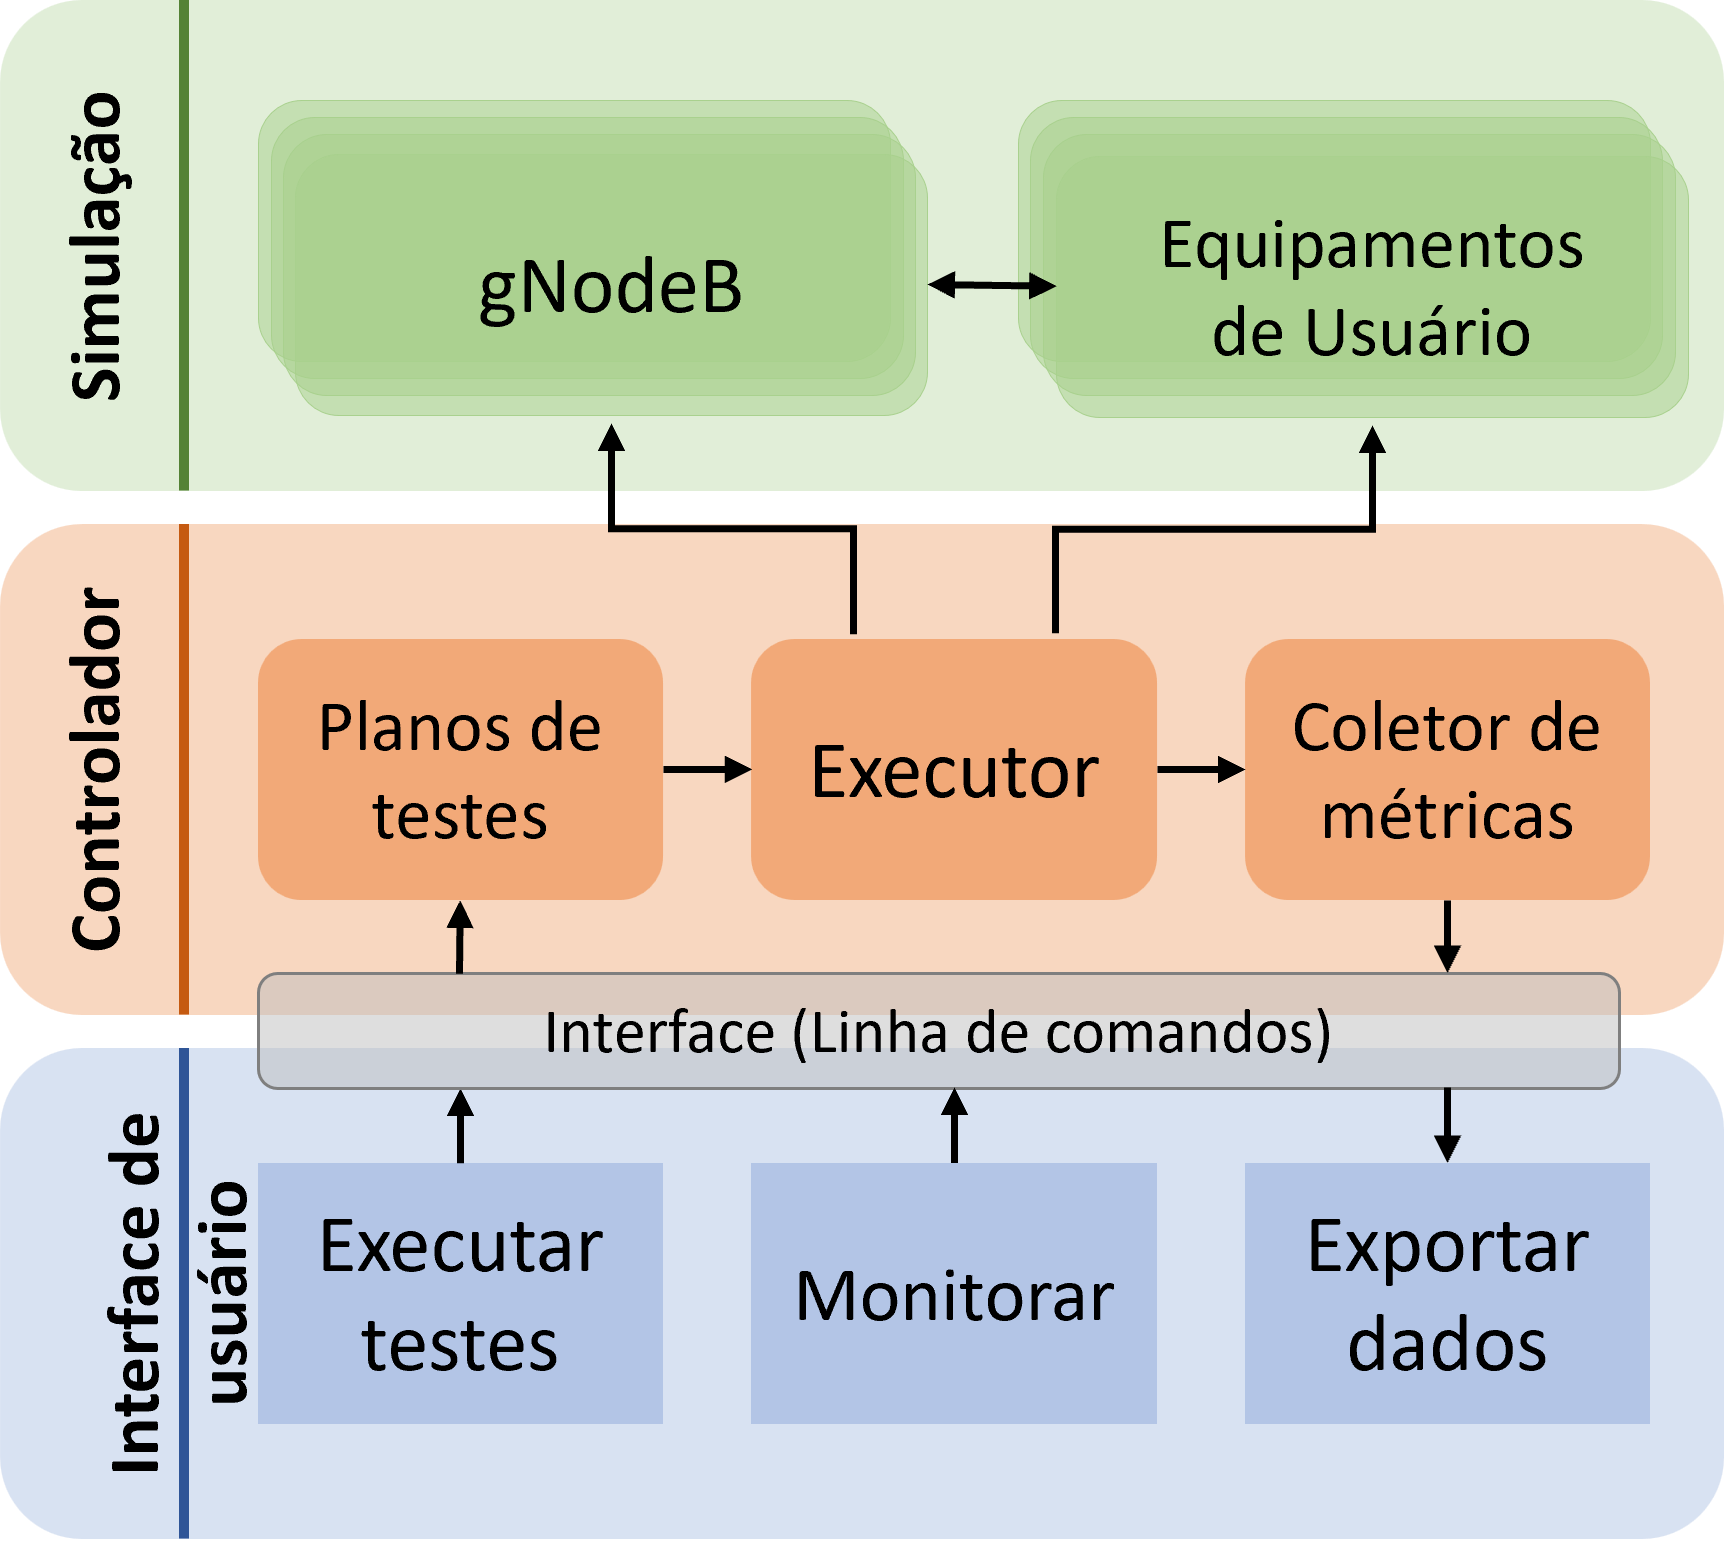
\includegraphics[width=0.6\textwidth]{TG2/Chapters/Soluction/Figures/Arquitetura-Componentes.png}
    \caption{Arquitetura do testador}
    \label{fig:tester_arch}
\end{figure}


Para desenvolver este trabalho, além do módulo implementado internamente no testador, também foi necessário desenvolver algumas ferramentas para a automação da criação e configuração do ambiente de testes e da execução dos experimentos. Essas ferramentas orquestram as múltiplas execuções dos experimentos e coletam os dados gerados para análise futura. A seguir, são apresentadas as ferramentas desenvolvidas no decorrer deste trabalho.

\subsection{Módulo de teste}

Para a execução de testes de desempenho, foi desenvolvido um módulo para o testador que permite a execução de múltiplas conexões de equipamentos de usuários simultâneas.
Esse módulo foi implementado suportando parâmetros de configuração para facilitar variações entre os testes. 
Desta forma, é possível definir o número de equipamentos de usuário a serem conectados, o atraso em milissegundos entre uma conexão e outra e o atraso em segundos para começar a execução do experimento.

No começo da execução, esse módulo simula uma gNodeB e inicia a conexão com o núcleo da rede. Após a conexão ser bem sucedida, é aguardado o tempo para iniciar a execução do experimento.
Ao iniciar o experimento, o módulo inicia um fluxo de trabalho em paralelo para criar uma nova instância de UE e realizar a conexão com o núcleo da rede.
Após iniciar o fluxo de trabalho em paralelo, o módulo aguarda o atraso entre conexões definido pelo usuário antes de iniciar o próximo fluxo, até que a quantidade de dispositivos definida seja atingida.

Durante a etapa de desenvolvimento do módulo, foi descoberta uma limitação na implementação do testador, que não consegue gerenciar mais que 255 UEs conectados simultaneamente.
Analisando o código, observa-se que a correção da limitação necessitaria de tempo e recursos não previstos na presente pesquisa.
Foi feito um contato com os desenvolvedores do testador sobre essa limitação, mas a solução para o problema não foi implementada até o presente momento.
Sendo assim, foi decidido criar múltiplas instâncias do testador, cada uma simulando uma gNodeB diferente, todas se conectando de forma simultânea na mesma instância do núcleo, cada uma simulando uma quantidade predefinida de UEs.
Desse modo, foi possível testar o comportamento de um núcleo de rede 5G com múltiplos UEs e gNodeB.

\subsection{Módulo de coleta de dados do testador}

O módulo de coleta de dados consiste em um fluxo de execução em paralelo que registra o tempo (em nanossegundos) que cada UE demorou para trocar entre cada estado da conexão com o núcleo da rede 5G.
As informações de tempo para cada estado de cada UE são escritas na saída de texto padrão do contêiner utilizado pela instância do testador.
Esse módulo foi implementado nesta presente pesquisa, visto que o testador não possuía suporte para a coleta dessa métrica até o presente momento.

Ao final da execução, uma aplicação foi desenvolvida para realizar o processamento das informações geradas através das diversas instâncias do testador, fazendo um pré processamento dos dados, ordenando eles com base no horário da inicialização do UE (em nanossegundos a partir do \textit{epoch time}\footnote{\textit{Epoch time} é uma unidade de medida de tempo contada a partir da data 1 de janeiro de 1970 às 00:00:00 UTC.}) e gerando um arquivo de texto separado por vírgulas, permitindo a fácil importação dos resultados através de programas de análise de dados.
Inicialmente, essa aplicação foi desenvolvida para coletar e processar os registros de uma única instância do testador, ordenando em ordem crescente pelo identificador do UE os dados no arquivo de saída.
Entretanto, foi necessário modificar essa aplicação para suportar múltiplas instâncias de testadores executando em paralelo e reordenar os dados do arquivo de saída, visto que a ordem de conexão dos dispositivos deixou de ser realizada em ordem crescente do identificador.

A aplicação consiste em um \textit{script} escrito na linguagem \textit{JavaScript}\footnote{https://developer.mozilla.org/pt-BR/docs/Web/JavaScript} que é executado dentro de um contêiner \textit{Docker}, evitando a instalação de um interpretador de \textit{JavaScript} diretamente na máquina que está executando os experimentos.

\subsection{Módulo de coleta de dados do núcleo}

O desenvolvimento deste módulo teve a contribuição dos bolsistas de iniciação científica do projeto PORVIR-5G.
Esse módulo consiste na implementação de um fluxo sobre uma instância da aplicação \textit{Node-RED}\footnote{https://nodered.org/}.

Um fluxo foi desenvolvido para listar todos os contêineres em execução na máquina e realizar a coleta das métricas do \textit{Docker} e armazená-las em uma instância do banco de dados \textit{InfluxDB}\footnote{https://www.influxdata.com/}. Esse fluxo foi definido para ser executado automaticamente após a inicialização do contêiner do \textit{Node-RED}, permitindo a coleta de dados de uso de disco, rede, processador, memória, entre outras, de forma automatizada pelo orquestrador do experimento.

\subsection{Orquestrador}
\label{sub:arch-orchestrator}

Com o objetivo de realizar todas as execuções dos experimentos de forma mais semelhante possível, foi desenvolvido um orquestrador que gerencia toda a execução do experimento.
O orquestrador consiste em uma série de roteiros de execução, desenvolvidos em sua maioria sobre as linguagens \textit{Bash Script} e \textit{JavaScript}.
A Figura \ref{fig:flux_orq} representa um fluxograma do algoritmo de execução do orquestrador.
O orquestrador é executado através de uma interface de usuário por linha de comandos, suportando diversos comandos para definir os parâmetros de execução do experimento, permitindo ao usuário automatizar a execução de experimentos de forma simplificada.

Os parâmetros suportados são a quantidade total de equipamentos de usuário a serem conectados no núcleo da rede, a quantidade de testadores que serão executados em paralelo, o tempo em milissegundos para ser aguardado entre cada conexão de equipamento de usuário, o tempo em segundos para aguardar a inicialização, qual núcleo da rede 5G deve ser utilizado para executar o experimento e qual experimento será executado.
Além dos parâmetros de execução do experimento, o orquestrador também permite o usuário interromper a última execução e limpar o ambiente de testes, removendo todos os contêineres e dados gerados pelo experimento, além de permitir executar o orquestrador em modo de depuração, exibindo para o usuário todos os registros de execução.

Ao iniciar a execução do orquestrador, será feita uma análise sobre o sistema operacional, verificando se a versão necessária do \textit{Kernel} do sistema está instalada.
Após realizar esta validação, o orquestrador irá verificar se todas as dependências estão corretamente instaladas e configuradas. Caso contrário, o orquestrador fará as devidas modificações automaticamente.
Uma vez que o sistema está pronto, é iniciada a execução do experimento desejado.
Primeiramente, o código-fonte do núcleo da rede 5G escolhido será baixado, compilado e seus arquivos binários serão armazenados em uma imagem de contêiner \textit{Docker}, que será iniciada na sequência.
Após a inicialização do núcleo, a base de dados desse núcleo é preenchida com as informações necessárias para a conexão dos UEs de acordo com as configurações do experimento.
Concluindo-se essa etapa, é iniciado o módulo de coleta de dados do núcleo, descrito anteriormente.
Por fim, inicia-se o contêiner do testador com os parâmetros definidos pelo usuário.

O orquestrador foi desenvolvido para suportar diferentes implementações de núcleos da rede 5G. Para isso, foi desenvolvida uma interface genérica para a inicialização do núcleo. Assim, para adicionar o suporte a um novo núcleo, basta implementar essa interface para o núcleo desejado e adicioná-la ao orquestrador.
Para a realização deste trabalho, foi desenvolvido o suporte para as implementações de núcleo 5G \textit{free5GC}, \textit{Open5GS} e \textit{OpenAirInterface}.
Todos os códigos fontes utilizados no desenvolvimento da presente pesquisa encontram-se no repositório do projeto PORVIR-5G\footnote{https://github.com/PORVIR-5G-Project} disponível através da plataforma \textit{GitHub}.

\begin{figure}[!ht]
    \centering
    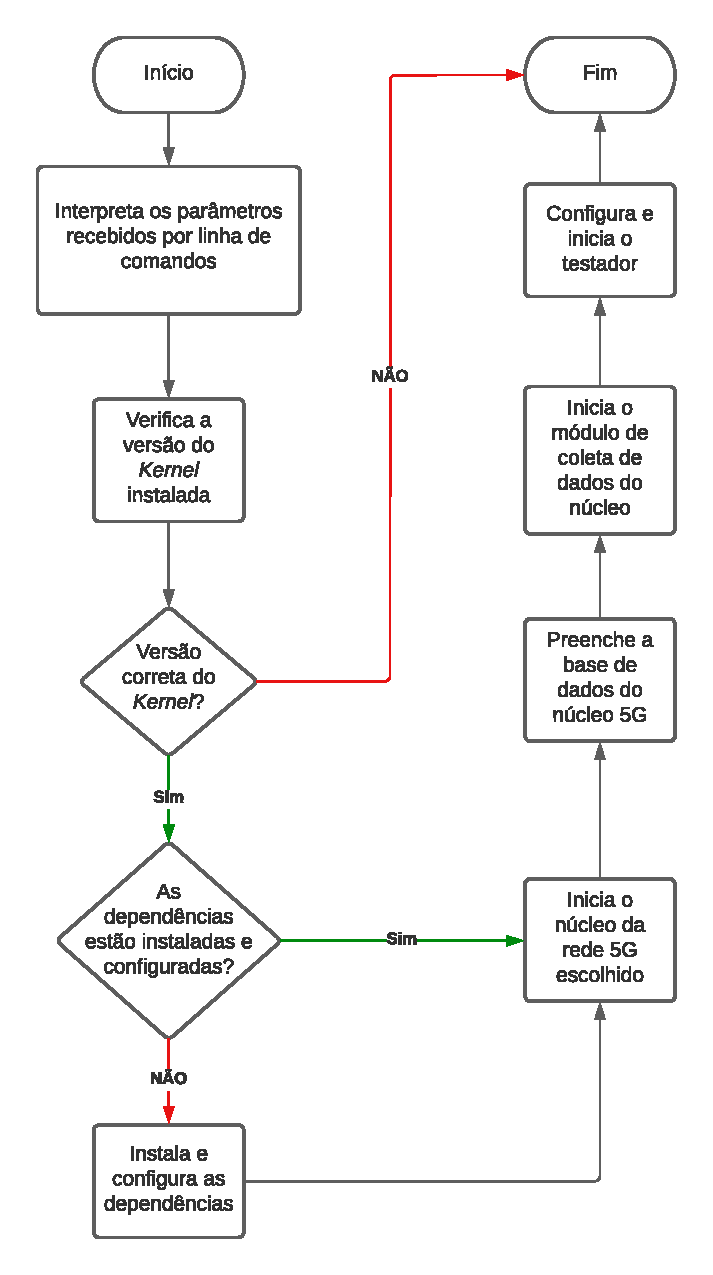
\includegraphics[width=0.55\textwidth]{TG2/Chapters/Soluction/Figures/Fluxograma-Orquestrador.pdf}
    \caption{Fluxograma de execução do orquestrador}
    \label{fig:flux_orq}
\end{figure}




% e aqui vai a parte principal
%
% \chapter{Estado da arte}
% \chapter{Mais estado da arte}
% \chapter{A minha contribuição}
% \chapter{Prova de que a minha contribuição é válida}
% \chapter{Conclusão}

% referencias
% aqui será usado o environment padrao `thebibliography'; porém, sugere-se
% seriamente o uso de BibTeX e do estilo abnt.bst (veja na página do
% UTUG)
%
% observe também o estilo meio estranho de alguns labels; isso é
% devido ao uso do pacote `natbib', que permite fazer citações de
% autores, ano, e diversas combinações desses

\bibliographystyle{abntex2-alf}
\bibliography{TG2/references,TG2/refs-3gpp,TG2/refs-web}

\end{document}
